

\section{Graph Basics}
\subsection{Motivation Problem}

\begin{frame}[fragile]
  \frametitle{Initial Problem: UVA 11902 -- Dominator}
  \begin{block}{}
    You are given a directed graph. Node {\bf A} dominates
    node {\bf B} if you \alert{must} pass {\bf B} to reach {\bf A}.
    \bigskip

    List the nodes that dominate each other.
  \end{block}
  \begin{center}
    \begin{columns}[T]
      \column{0.4\textwidth}
      \begin{tikzpicture}[scale=1.3,auto,swap]
  \tikzset{edge/.style = {->,>=latex'}}
  \node[vertex] (a) at (0,0) {0};
  \node[vertex] (b) at (1,1) {1};
  \node[vertex] (c) at (1,-1) {2};
  \node[vertex] (d) at (2,0) {3};
  \node[vertex] (e) at (3,0) {4};
  \draw[edge] (a) to (b);
  \draw[edge] (a) to (c);
  \draw[edge] (b) to (d);
  \draw[edge] (c) to (d);
  \draw[edge] (d) to (e);
\end{tikzpicture}

      \column{0.3\textwidth}
      {\bf Input}
\begin{verbatim}
1
5
0 1 1 0 0
0 0 0 1 0
0 0 0 1 0
0 0 0 0 1
0 0 0 0 0
\end{verbatim}
\column{0.3\textwidth}
{\bf Output}
{\small
\begin{verbatim}
Case 1:
+---------+
|Y|Y|Y|Y|Y|
+---------+
|N|Y|N|N|N|
+---------+
|N|N|Y|N|N|
+---------+
|N|N|N|Y|Y|
+---------+
|N|N|N|N|Y|
+---------+
\end{verbatim}}
    \end{columns}
  \end{center}
  %% Simple graph problems (quick modification of DFS/BFS)
  % Dominator: UVA 11902 - Page 148
\end{frame}


\begin{frame}
  \frametitle{Initial Problem: UVA 11902 -- Dominator}
  \begin{block}{}
    What do we need to do to solve this problem?
  \end{block}

  \begin{center}
    \begin{columns}[T]
      \column{0.5\textwidth}
      \begin{tikzpicture}[scale=1.3,auto,swap]
  \tikzset{edge/.style = {->,>=latex'}}
  \node[vertex] (a) at (0,0) {0};
  \node[vertex] (b) at (1,1) {1};
  \node[vertex] (c) at (1,-1) {2};
  \node[vertex] (d) at (2,0) {3};
  \node[vertex] (e) at (3,0) {4};
  \draw[edge] (a) to (b);
  \draw[edge] (a) to (c);
  \draw[edge] (b) to (d);
  \draw[edge] (c) to (d);
  \draw[edge] (d) to (e);
\end{tikzpicture}

      \column{0.5\textwidth}
      \begin{itemize}
        \item Represent the graph as a data structure;\bigskip
        \item Find the relationship between the nodes;\bigskip
        \item Determine which nodes "dominate" each other;\bigskip
      \end{itemize}
    \end{columns}
  \end{center}
  %% Simple graph problems (quick modification of DFS/BFS)
  % Dominator: UVA 11902 - Page 148
\end{frame}

\subsection{Structure and Representation}

\begin{frame}
  \frametitle{Base definition}

  \begin{block}{}
    A \structure{graph} $G = {V,E}$ is defined as a set of
    \structure{vertices} $V$, and \structure{edges} $E$. Each edge
    connects exactly two vertices.
  \end{block}
  {\smaller

    \begin{columns}[T]
      \column{0.6\textwidth}
      \begin{itemize}
      \item Edges can be \structure{directed} or \structure{undirected};
      \item Edges and can be \structure{weighted} (and sometimes vertices too!);
      \item Edges can be \structure{self-edges}, and/or \structure{multiple edges}
      \end{itemize}

      \bigskip

      Graph Problems:
      \begin{itemize}
      \item Find a vertex or edge with a certain characteristic;
      \item Find a relationship between vertices or edges;
      \end{itemize}

      \column{0.4\textwidth}


      \begin{tikzpicture}[scale=.8,auto,swap]
        \tikzset{edge/.style = {->,>=latex'}}
        \node[vertex] (a) at (0,0) {};
        \node[vertex] (b) at (2,3) {};
        \node[vertex] (c) at (4,2) {};
        \node[vertex] (d) at (4,0) {};
        \draw[edge] (a) to (b);
        \draw[edge] (a) to[bend left] (c);
        \draw[edge] (c) to[bend left] (a);
        \draw[edge] (d) to (c);
        \draw[edge] (d) to[loop left] (d);
        \draw[edge] (d) to[loop right] (d);
      \end{tikzpicture}

      \vspace{.5cm}

      \begin{tikzpicture}[scale=1,auto,swap]
        \node[vertex] (a) at (0,2) {a};
        \node[vertex] (b) at (0,0) {b};
        \node[vertex] (c) at (2,1) {c};
        \node[vertex] (d) at (4,0) {d};
        \node[vertex] (e) at (4,1) {e};
        \draw[edge] (a) -- node[weight] {$7$} (b);
        \draw[edge] (b) -- node[weight] {$-2$} (c);
        \draw[edge] (c) -- node[weight] {$3$} (a);
        \draw[edge] (c) -- node[weight] {$5$} (d);
      \end{tikzpicture}

    \end{columns}
  }
\end{frame}

\begin{frame}[fragile]
  \frametitle{How do we implement a graph?}
  \begin{block}{Adjacency Matrix - Connection between Vertices}
\begin{verbatim}
int adj[100][100];

for (int i = 0; i < n; i++)
  for (int j = 0; i < n; j++)
    cin >> adj[i][j]; // 0 if no edge, 1 if edge
\end{verbatim}

    \begin{itemize}
    \item \structure{Pro}: Very simple to program;
    \item \alert{Con}:
      \begin{itemize}
      \item Cannot store multigraph;
      \item Waste space for sparse graphs;
      \item Time $O(V)$ to calculate number of neighbors;
      \end{itemize}
    \end{itemize}
  \end{block}
\end{frame}

\begin{frame}[fragile]
  \frametitle{How do we implement a graph?}

  {\smaller
  \begin{block}{Vector-Edge List -- Stores Edges list for each Vertex}
\begin{verbatim}

typedef pair<int,int> edge; // <destination, weight> pair
typedef vector<edge> neighb;// all the neighbors of one V
vector<neighb> AdjList;     // all vertices

int e;
for (int i = 0; i < n; i++)
  for (int j = 0; j < n; j++)
    cin >> e;
    if (e == 1)
      AdjList[i].push_back(pair(j,1));

\end{verbatim}

    \begin{itemize}
    \item \structure{Pro}: $O(V+E)$ space, efficient if
      graph is sparse; Can store multigraph;
    \item \alert{Con}: Code is more complex
      than adjacency list; $O(\text{log}V)$
      to test if two vertices are adjacent.
    \end{itemize}
  \end{block}
  }
\end{frame}

\begin{frame}[fragile]
  \frametitle{How do we implement a graph?}
  \begin{block}{Edge List}
\begin{verbatim}

pair <int,int> edge; // Edge between i and j
vector<pair <int,ii>> Elist; // Store edges;

int e;
for (int i = 0; i < n; i++)
  for (int j = 0; j < n; j++)
    cin >> e;
    if (e == 1)
      Elist.push_back(pair(1, pair(i,j)));
\end{verbatim}
\end{block}
    \vfill

    \begin{itemize}
    \item Used by \structure{Kruskal's Algorithm}, among others.
    \item Some algorithms require specialized data structures.
    \item Use arrays to save data about vertices.
    \end{itemize}
\end{frame}


\subsection{BFS, DFS}
\begin{frame}
  \frametitle{Graph Search: BFS and DFS}
    \begin{itemize}
    \item Almost every Graph algorithm uses BFS or DFS;
    \item Learn to do this with your eyes closed;
    \end{itemize}

  \begin{block}{Depth First Search -- DFS}
    \begin{itemize}
    \item Easy to implement using Recursion;
    \item Visit first edge of each vertice until you find a loop;
    \end{itemize}
  \end{block}

  \begin{block}{Breadth First Search -- BFS}
    \begin{itemize}
    \item Easy to implement using loops, requires keeping track of
      visited vertices on a queue;
    \item Put edge/vertice on a FIFO queue, then visit next;
    \end{itemize}
  \end{block}
\end{frame}

\begin{frame}
  \frametitle{BFS/DFS: Visualization}
  \begin{columns}[t]
    \column{0.5\textwidth}
    \begin{exampleblock}{DFS}
      \vspace{0.1cm}
      \begin{center}
      \begin{tikzpicture}[scale=1.3,auto,swap]
        \node[vertex] (a) at (0,0) {};
        \node[vertex] (b) at (2,0) {};
        \node[vertex] (c) at (0,-1) {};
        \node[vertex] (d) at (1,-2) {};
        \node[vertex] (e) at (0,-2) {};
        \node[vertex] (f) at (2,-2) {};
        \node[vertex] (g) at (2,-3) {};
        \node[vertex] (h) at (1,-4) {};
        \draw[edge] (a) to (b);
        \draw[edge] (a) to (c);
        \draw[edge] (a) to (f);
        \draw[edge] (b) to (f);
        \draw[edge] (c) to (d);
        \draw[edge] (c) to (e);
        \draw[edge] (f) to (h);
        \draw[edge] (e) to (h);
        \draw[edge] (f) to (g);
        \draw<2->[red edge] (a) to (b);
        \draw<3->[red edge] (b) to (f);
        \draw<4->[red edge] (f) to (g);
        \draw<5->[red edge] (f) to (h);
        \draw<6->[red edge] (h) to (e);
        \draw<7->[red edge] (e) to (c);
        \draw<8->[red edge] (c) to (d);
      \end{tikzpicture}
      \end{center}
      \vspace{0.1cm}
    \end{exampleblock}
    \column{0.5\textwidth}
    \begin{block}{BFS}
      \vspace{0.1cm}
      \begin{center}
      \begin{tikzpicture}[scale=1.3,auto,swap]
        \node[vertex] (a) at (0,0) {};
        \node[vertex] (b) at (2,0) {};
        \node[vertex] (c) at (0,-1) {};
        \node[vertex] (d) at (1,-2) {};
        \node[vertex] (e) at (0,-2) {};
        \node[vertex] (f) at (2,-2) {};
        \node[vertex] (g) at (2,-3) {};
        \node[vertex] (h) at (1,-4) {};
        \draw[edge] (a) to (b);
        \draw[edge] (a) to (c);
        \draw[edge] (a) to (f);
        \draw[edge] (b) to (f);
        \draw[edge] (c) to (d);
        \draw[edge] (c) to (e);
        \draw[edge] (f) to (h);
        \draw[edge] (e) to (h);
        \draw[edge] (f) to (g);
        \draw<2->[red edge] (a) to (b);
        \draw<3->[red edge] (a) to (f);
        \draw<4->[red edge] (a) to (c);
        \draw<5->[red edge] (f) to (g);
        \draw<6->[red edge] (f) to (h);
        \draw<7->[red edge] (c) to (d);
        \draw<8->[red edge] (c) to (e);
      \end{tikzpicture}
      \end{center}
      \vspace{0.1cm}
    \end{block}
  \end{columns}
\end{frame}

\begin{frame}[fragile]
  \frametitle{DFS Implementation}
  \begin{exampleblock}{DFS with adjacency list}
\begin{verbatim}
#define UNVISITED 0
#define VISITED 1
vector<int> dfs_vis; // list visited nodes

void dfs(int v) {
   dfs_vis[v] = VISITED;
   for (int i; i < (int) Adj_list[v].size(); i++)
   {
      pair <int,int> u = Adj_list[v][i];
      if (dfs_vis[u.first] == UNVISITED)
         dfs(v.first); // else -- Found Loop!
   }
}
dfs(1);
\end{verbatim}
  \end{exampleblock}
\end{frame}

\begin{frame}[fragile]
  \frametitle{BFS Implementation}
  \begin{exampleblock}{BFS with adjacency matrix ($O(N^2)$!)}
\begin{verbatim}
#define INF 1000000 // Not visited
int s = 1; // Search started

vector<int> d(N,INF); d[s] = 0;  // Distances
queue<int> q; q.push(s);
while(!q.empty()) {
  int u = q.front(); q.pop();
  for (int i=0; i < N; i++) {
    if (adj[u][i] && d[i] == INF) {
      d[i] = d[u] + 1;     // Update Distance
      q.push(i);
    }
  }
}
\end{verbatim}
  \end{exampleblock}
\end{frame}

\subsection{Back to the Dominator}

\begin{frame}[fragile]
  \frametitle{Back to the Dominator Problem}

  {\smaller
  \begin{exampleblock}{Thinking about the problem again}
    X is \structure{Dominated} by Y if \structure{all paths} from
    the root to Y go through X.

    \bigskip
  \end{exampleblock}}

  \begin{center}
    \begin{tikzpicture}[scale=0.9,auto,swap]
      \tikzset{edge/.style = {->,>=latex'}}
      \node[vertex] (a) at (0,0) {0};
      \node[vertex] (b) at (1,1) {1};
      \node[vertex] (c) at (1,-1) {2};
      \node[vertex] (d) at (2,0) {3};
      \node[vertex] (e) at (3,0) {4};
      \draw[edge] (a) to (b);
      \draw[edge] (a) to (c);
      \draw[edge] (b) to (d);
      \draw[edge] (c) to (d);
      \draw[edge] (d) to (e);
    \end{tikzpicture}
  \end{center}
\end{frame}

\begin{frame}[fragile]
  \frametitle{Back to the Dominator Problem}

  {\smaller
  \begin{exampleblock}{$N^2$ solution: DFS $N$ times}
\begin{verbatim}
def DFS2(S,P): ...  // Modified DFS: never visits P;

DFS2(0,-1)
Mark every VISITED vertex as DOMINATED by 0

for i in (1:N):
   reset VISITED array
   DFS2(0,i)
   For every NOT-VISITED vertex j:
      if j is DOMINATED by 0:
         j is DOMINATED by i
\end{verbatim}
  \end{exampleblock}}

  \begin{center}
    \begin{tikzpicture}[scale=0.7,auto,swap]
      \tikzset{edge/.style = {->,>=latex'}}
      \node[vertex] (a) at (0,0) {0};
      \node[vertex] (b) at (1,1) {1};
      \node[vertex] (c) at (1,-1) {2};
      \node[vertex] (d) at (2,0) {3};
      \node[vertex] (e) at (3,0) {4};
      \draw[edge] (a) to (b);
      \draw[edge] (a) to (c);
      \draw[edge] (b) to (d);
      \draw[edge] (c) to (d);
      \draw[edge] (d) to (e);
    \end{tikzpicture}
  \end{center}
\end{frame}



%%%%%%%%%%%%%%%%%%%%%%%%%%%%%%%%%%%%%%%%%%%%%%%%%%%%%%%%%%%%%%%%%%%%%%%%%%%%%%%
%% \subsection{Graph Terms}
%% \begin{frame}
%%   \frametitle{Quick Review of Graph Terms (1)}
%%   {\smaller
%%     \begin{block}{}
%%       You probably know all of these. If not, ask questions!
%%     \end{block}

%%     \begin{columns}[T]
%%       \column{0.6\textwidth}
%%       \begin{itemize}
%%       \item A Graph $G$ is made of a set of \structure{vertices} $V$
%%         and \structure{edges} $E$.
%%       \item Edges can be \structure{directed}\\ (has source and destination vertices);
%%       \item Edges can be \structure{weighted} or not\\ (all weigths = 1);
%%       \item Sets of nodes can be \structure{connected}\\ or \structure{disconnected}
%%       \item Directed Graphs can be \structure{Strongly Connected}
%%       \item Edges can be \structure{self-edges}, and/or \structure{multiple edges}
%%       \end{itemize}
%%       \column{0.4\textwidth}

%%       \begin{tikzpicture}[scale=.8,auto,swap]
%%         \tikzset{edge/.style = {->,>=latex'}}
%%         \node[vertex] (a) at (0,0) {};
%%         \node[vertex] (b) at (2,3) {};
%%         \node[vertex] (c) at (4,2) {};
%%         \node[vertex] (d) at (4,0) {};
%%         \draw[edge] (a) to (b);
%%         \draw[edge] (a) to[bend left] (c);
%%         \draw[edge] (c) to[bend left] (a);
%%         \draw[edge] (d) to (c);
%%         \draw[edge] (d) to[loop left] (d);
%%         \draw[edge] (d) to[loop right] (d);
%%       \end{tikzpicture}

%%       \vspace{.5cm}

%%       \begin{tikzpicture}[scale=1,auto,swap]
%%         \node[vertex] (a) at (0,2) {a};
%%         \node[vertex] (b) at (0,0) {b};
%%         \node[vertex] (c) at (2,1) {c};
%%         \node[vertex] (d) at (4,0) {d};
%%         \node[vertex] (e) at (4,1) {e};
%%         \draw[edge] (a) -- node[weight] {$7$} (b);
%%         \draw[edge] (b) -- node[weight] {$-2$} (c);
%%         \draw[edge] (c) -- node[weight] {$3$} (a);
%%         \draw[edge] (c) -- node[weight] {$5$} (d);
%%       \end{tikzpicture}

%%     \end{columns}
%%   }
%% \end{frame}

%% \begin{frame}
%%   \frametitle{Quick Review of Graph Terms (2)}

%%   {\smaller
%%     \begin{block}{}
%%       You probably know all of these. If not, ask questions!
%%     \end{block}

%%     \begin{columns}[T]
%%       \column{0.6\textwidth}
%%       \begin{itemize}
%%       \item A \structure{path} is a set of vertices connected by edges;
%%       \item A \structure{cycle} is a path with first and last vertices identical;
%%       \item \structure{Labelled} graphs and \structure{Isomorphic} graphs;
%%       \item A \structure{tree} is a acyclical, undirected graph;
%%       \item A \structure{spanning tree} is a subset of edges from E'
%%         that form a tree, connecting all nodes $V \in G$;
%%       \item A \alert{spamming tree} houses very noisy insects in summer;
%%       \end{itemize}
%%       \column{0.4\textwidth}
%%       \begin{tikzpicture}[scale=1,auto,swap]
%%         \node[vertex] (s) at (0,0) {a};
%%         \node[vertex] (a1) at (-1,-1) {b};
%%         \node[vertex] (a2) at (1,-1) {c};
%%         \node[vertex] (b1) at (-1,-2) {d};
%%         \node[vertex] (b2) at (0,-2) {e};
%%         \draw[edge] (s) to (a1);
%%         \draw[edge] (s) to  (a2);
%%         \draw[edge] (a1) to  (b1);
%%         \draw[edge] (a1) to  (b2);
%%         \draw[black edge] (b1) to (b2);
%%         \draw[black edge] (a2) to (b2);
%%       \end{tikzpicture}

%%       \vspace{.5cm}

%%       \begin{tikzpicture}[scale=1,auto,swap]
%%         \node[vertex] (s) at (0,0) {e};
%%         \node[vertex] (a1) at (-1,-1) {d};
%%         \node[vertex] (a2) at (1,-1) {b};
%%         \node[vertex] (b1) at (-1,-2) {c};
%%         \node[vertex] (b2) at (0,-2) {a};
%%         \draw[edge] (s) to (a1);
%%         \draw[edge] (s) to  (a2);
%%         \draw[edge] (a1) to  (b1);
%%         \draw[edge] (a1) to  (b2);
%%         \draw[black edge] (b1) to (b2);
%%         \draw[black edge] (a2) to (b2);
%%       \end{tikzpicture}
%%   \end{columns}}

%% \end{frame}

%% \begin{frame}
%%   \frametitle{Quick Review of Graph Terms (3)}

%%   {\smaller
%%     \begin{block}{}
%%       You probably know all of these. If not, ask questions!
%%     \end{block}

%%     \begin{columns}[T]
%%       \column{0.6\textwidth}
%%       \begin{itemize}
%%       \item The \structure{degree} of a node is the number of edges
%%         connected to it;
%%       \item Directed graphs have \structure{in-degrees} and
%%         \structure{out-degrees};
%%       \item A \structure{bipartite} graph can be divided in two sets
%%         of unconnected vertices;
%%       \item A \structure{Match} or \structure{Pairing} is a set of
%%         edges that connects the nodes in the bipartite graph;
%%       \end{itemize}
%%       \column{0.4\textwidth}
%%       \begin{tikzpicture}[scale=.8,auto,swap]
%%         \node[vertex] (a) at (0,0) {deg: 2};
%%         \node[vertex] (b) at (2,1) {};
%%         \node[vertex] (c) at (2,-1) {};
%%         \node[vertex] (d) at (4,0) {in,out:1};
%%         \draw[edge] (a) to (b);
%%         \draw[edge] (a) to (c);
%%         \tikzset{edge/.style = {->,>=latex'}}
%%         \draw[edge] (c) to (d);
%%         \draw[edge] (d) to (b);
%%       \end{tikzpicture}

%%       \vspace{.5cm}

%%       \begin{tikzpicture}[scale=.8,auto,swap]
%%         \node[vertex] (a1) at (0,0) {};
%%         \node[vertex] (b1) at (0,2) {};
%%         \node[vertex] (a2) at (1,0) {};
%%         \node[vertex] (b2) at (2,2) {};
%%         \node[vertex] (a3) at (3,0) {};
%%         \node[vertex] (b3) at (3,2) {};
%%         \node[vertex] (a4) at (5,0) {};
%%         \node[vertex] (b4) at (4,2) {};
%%         \draw[red edge] (a1) to (b1);
%%         \draw[red edge] (a2) to (b3);
%%         \draw[red edge] (a3) to (b4);
%%         \draw[red edge] (a4) to (b2);
%%         \draw[edge] (a1) to (b1);
%%         \draw[edge] (a1) to (b2);
%%         \draw[edge] (a2) to (b1);
%%         \draw[edge] (a2) to (b3);
%%         \draw[edge] (a2) to (b4);
%%         \draw[edge] (a3) to (b1);
%%         \draw[edge] (a3) to (b4);
%%         \draw[edge] (a4) to (b3);
%%         \draw[edge] (a4) to (b2);
%%       \end{tikzpicture}
%%   \end{columns}}
%% \end{frame}


\section{Common Algorithms}
\subsection{Connected Components}
\begin{frame}[fragile]
  \frametitle{Common Algorithms Using DFS/BFS}
  {\smaller
    \begin{exampleblock}{}
      With small modifications to BFS/DFS, we can solve many simple problems
    \end{exampleblock}

    \vfill

    \begin{block}{Problem Example: Extra cables}
      You own a network of $N$ computers;

      \bigskip

      You have a list of every pair of computers connected by cable ($i,j$)

      \bigskip

      You need to buy $M$ extra cables to connect ALL computers. How
      many cables do you need?
    \end{block}
  }
\end{frame}

\begin{frame}
  \frametitle{Common Algorithms Using DFS/BFS}
  \framesubtitle{Connected Components}

  This problem is defined in graph theory as finding
  \structure{Connected Components}.

  \begin{center}
    \begin{tikzpicture}[scale=1,auto,swap]
      \node[vertex] (a) at (0,2) {a};
      \node[vertex] (b) at (0,0) {b};
      \node[vertex] (c) at (2,1) {c};
      \node[vertex] (d) at (4,0) {d};
      \node[vertex] (e) at (4,1) {e};
      \node[vertex] (1) at (8,2) {1};
      \node[vertex] (2) at (9,0) {2};
      \draw[edge] (a) to (b);
      \draw[edge] (b) to (c);
      \draw[edge] (c) to (a);
      \draw[edge] (c) to (d);
      \draw[edge] (1) to (2);
    \end{tikzpicture}
  \end{center}
\end{frame}

\begin{frame}[fragile]
  \frametitle{Common Algorithms Using DFS/BFS}
  \framesubtitle{Connected Components}

  {\smaller
    One way to find all connected components, is to repeat
    a BFS (or DFS) until all nodes are visited.

    \begin{exampleblock}{}
\begin{verbatim}
int cables = 0;
// dfs(x) from slide 11

for (int = 0; i < N; i++)
   if (dfs_vis[i] == UNVISITED) // New unvisited!
   {
      dfs(i);                   // Visit some vertices
      cables += 1;
   }
cout << cables - 1 << "\n";
\end{verbatim}
    \end{exampleblock}}

\begin{center}
  \begin{tikzpicture}[scale=1,auto,swap]
    \node[vertex] (a) at (0,0) {0};
    \node[vertex] (b) at (0,1) {1};
    \node[vertex] (c) at (1,0) {2};
    \node[vertex] (d) at (1,1) {3};
    \node[vertex] (e) at (2,0) {4};
    \node[vertex] (f) at (2,1) {5};
    \draw[edge] (a) to (b);
    \draw[edge] (a) to (c);
    \draw[edge] (b) to (c);
    \draw[edge] (d) to (f);
  \end{tikzpicture}
\end{center}
\end{frame}

\begin{frame}
  \frametitle{Common Algorithms Using DFS/BFS}
  \framesubtitle{Connected Components}

  We can also find the connected components using \alert{UFDS}.

  \bigskip

  How would you implement it?
\end{frame}

\subsection{Flood Fill}

\begin{frame}[fragile]
  \frametitle{More Common Algorithms Using DFS/BFS}
  \framesubtitle{Is this a graph problem?}

  \begin{block}{Problem: The Biggest Island}
    You want to build a new castle in the game of CraftMine. For this,
    you need to find the biggest island in the world map.

    \bigskip

    \structure{Input:} The following 2D map of the map:
\begin{verbatim}
....................................
.###.......###.....#.....###.####...
.#####....#####.##.#####.##....#....
.###........###..#...##..#....###...
......###.......###...####...##.....
....####.............######.....###.
....####.......#.......###......###.
....................................
\end{verbatim}
  \end{block}

  \bigskip

  Is this even a graph???
\end{frame}

\begin{frame}
  \frametitle{More Common Algorithms Using DFS/BFS}
  \framesubtitle{Implicit Graphs and Floodfill}


  \begin{columns}
    \column{0.7\textwidth}
    {\smaller
    \begin{itemize}
    \item \structure{Implict Graphs} suggest graph organization;
    \item But it is not necessary to store the vertices and edges;
    \item \structure{Example:} Game boards; Distances; Grids;

      \bigskip

    \item No graph Structure, but same graph algorithms;
    \end{itemize}
    }
    \column{0.3\textwidth}
    \begin{tikzpicture}[scale=1,auto,swap]
      \node[vertex] (00) at (0,0) {};
      \node[vertex] (01) at (0,1) {};
      \node[vertex] (02) at (0,2) {};
      \node[vertex] (03) at (0,3) {};
      \node[vertex] (04) at (0,4) {};
      \node[vertex] (05) at (0,5) {};
      \node[vertex] (10) at (1,0) {};
      \node[vertex] (11) at (1,1) {};
      \node[vertex] (12) at (1,2) {};
      \node[vertex] (13) at (1,3) {};
      \node[vertex] (14) at (1,4) {};
      \node[vertex] (15) at (1,5) {};
      \node[vertex] (20) at (2,0) {};
      \node[vertex] (21) at (2,1) {};
      \node[vertex] (22) at (2,2) {};
      \node[vertex] (23) at (2,3) {};
      \node[vertex] (24) at (2,4) {};
      \node[vertex] (25) at (2,5) {};
      \draw[edge] (00) to (01);\draw[edge] (00) to (10);
      \draw[edge] (01) to (02);\draw[edge] (01) to (11);
      \draw[edge] (02) to (03);\draw[edge] (02) to (12);
      \draw[edge] (03) to (04);\draw[edge] (03) to (13);
      \draw[edge] (04) to (05);\draw[edge] (04) to (14);
      \draw[edge] (10) to (11);\draw[edge] (10) to (20);
      \draw[edge] (11) to (12);\draw[edge] (11) to (21);
      \draw[edge] (12) to (13);\draw[edge] (12) to (22);
      \draw[edge] (13) to (14);\draw[edge] (13) to (23);
      \draw[edge] (14) to (15);\draw[edge] (14) to (24);
      \draw[edge] (20) to (21);\draw[edge] (21) to (22);
      \draw[edge] (22) to (23);\draw[edge] (23) to (24);
      \draw[edge] (24) to (25);\draw[edge] (15) to (25);
      \draw[edge] (05) to (15);
    \end{tikzpicture}
  \end{columns}

\end{frame}


\begin{frame}[fragile]
  \frametitle{Flood Fill}
  {\smaller
      We can solve the ``Biggest Island'' problem with
      \structure{Flood Fill}, which is just a variation of
      BFS/DFS for grids.

  \begin{exampleblock}{}
\begin{verbatim}
int dr[] = {1,1,0,-1,-1,-1,0,1}; // trick to explore an
int dc[] = {0,1,1,1,0,-1,-1,-1}; // implicit NESW graph

int floodfill(int y, int x) {
  if (y < 0 || y >= R || x < 0 || x >= C) return 0;
  if (grid[y][x] != '#') return 0;
  int ans = 1;
  grid[y][x] = '.';              // CHANGE the map
  for (int d = 0; d < 8; d++)
     ans += floodfill(y+dr[d], x+dc[d]);
  return ans;
}
\end{verbatim}
  \end{exampleblock}
  }
\end{frame}

\subsection{Topological Sort}

\begin{frame}[fragile]
  \frametitle{Another Classical Problem}
  \framesubtitle{Preparing a Course Curriculum}
  {\smaller
  \begin{block}{Problem Outline}
    You are a teacher and you have to prepare a course curriculum.
    You have a list of topics, but some topics are pre-requisite to others.

    \bigskip

    \structure{Input}: M, N, The list of M topics, followed by N ordered pairs of topics.

    \structure{Output}: A sorted list with all topics.

  \end{block}
\begin{verbatim}
5 4 Graphs DP Search Flow Programming
Programming Search
Search DP
Graph Flow
Search Graph


=====================
Result: Programming Search DP Graph Flow
\end{verbatim}

  }
\end{frame}

\begin{frame}
  \frametitle{Another Classical Problem}
  \framesubtitle{Topological sort}

  \begin{itemize}
  \item A \structure{directed} graph has a \structure{topological
    sort} if it has \alert{no cycles};
  \item We can use the \structure{in-degrees} and
    \structure{out-degrees} to calculate the topological sort;
  \end{itemize}

  \begin{center}
    \begin{tikzpicture}[scale=.8,auto,swap]
      \node[vertex] (a) at (0,0) {out: 2};
      \node[vertex] (b) at (2,1) {};
      \node[vertex] (c) at (2,-1) {};
      \node[vertex] (d) at (4,0) {in: 2 out:1};
      \node[vertex] (e) at (6,0) {};
      \tikzset{edge/.style = {->,>=latex'}}
      \draw[edge] (a) to (b);
      \draw[edge] (a) to (c);
      \draw[edge] (c) to (d);
      \draw[edge] (b) to (d);
      \draw[edge] (d) to (e);
    \end{tikzpicture}
  \end{center}
\end{frame}

\begin{frame}[fragile]
  \frametitle{Topological Sort (Directed Acyclic Graphs)}

  {\smaller

    \begin{exampleblock}{Khan's algorithm for Topological sort (modified edge-BFS)}
\begin{verbatim}
Q = queue(); toposort = list();
for j in edge:
   in_degree[j.destination] += 1
for i in node:                      // Start nodes to queue
   if in_degree[i] == 0: Q.add(i);
while (Q.size() > 0):
   u = Q.dequeue(); toposort.add(u);
   for i in u.out_edges():          // reduce in-degree
       v = i.destination
       in_degree[v] =- 1
       if in_degree[v] == 0:        // new start node
          Q.add(v);
\end{verbatim}
    \end{exampleblock}
  }
\end{frame}

\begin{frame}
  \frametitle{Topological Sort and Bottom-Up Dynamic Programming}

  %TODO
  What is the relationship between Topological Sort and Bottom-up DP?

  \bigskip

  Bottom-up DP are Topological sorts on Tables!
\end{frame}

\subsection{Bipartite Checking}

\begin{frame}[fragile]
  \frametitle{Bipartite Check}
  {\smaller
  To check whether a graph is bipartite, we perform a BFS or DFS on the graph,
  and set the color of every node to black or white, alternatively. Pay
  attention to collision conditions.

  \begin{exampleblock}{}
\begin{verbatim}
queue<int> q; q.push(s);
vector<int> color(V,INF); color[s] = 0;
bool isBipartite = true;
while (!q.empty() && isBipartite) {
   int u = q.front(); q.pop();
   for (int j=0; j < adj_list[u].size(); j++) {
      pair<int,int> v = adj_list[u][j];
      if (color[v] == INF) {
         color[v.first] = 1 - color[i];
         q.push(v.first);}
      else if (color[v.first] == color[u]) {
         isBipartite = False;
}}}
\end{verbatim}
  \end{exampleblock}
  }
\end{frame}

\begin{frame}
  \frametitle{Bipartite Check -- Visualization}
  \begin{columns}[t]
    \column{0.5\textwidth}
    \begin{exampleblock}{Testing Bipartite property}
      \vspace{0.1cm}
      \begin{center}
        \begin{tikzpicture}[scale=1.3,auto,swap]
          \node[vertex] (a) at (0,0) {};
          \node[vertex] (b) at (2,0) {};
          \node[vertex] (c) at (0,-1) {};
          \node[vertex] (d) at (1,-2) {};
          \node[vertex] (e) at (0,-2) {};
          \node[vertex] (f) at (2,-2) {};
          \node[vertex] (g) at (2,-3) {};
          \node[vertex] (h) at (1,-4) {};
          \draw[edge] (a) to (b);
          \draw[edge] (a) to (c);
          \draw[edge] (b) to (f);
          \draw[edge] (c) to (d);
          \draw[edge] (c) to (e);
          \draw[edge] (f) to (h);
          \draw[edge] (e) to (h);
          \draw[edge] (f) to (g);
          \uncover<2->{\node[red vertex] (a1) at (0,0) {};}
          \uncover<3->{\node[blue vertex] (b1) at (2,0) {};}
          \uncover<3->{\node[blue vertex] (c1) at (0,-1) {};}
          \uncover<4->{\node[red vertex] (d1) at (1,-2) {};}
          \uncover<4->{\node[red vertex] (e1) at (0,-2) {};}
          \uncover<4->{\node[red vertex] (f1) at (2,-2) {};}
          \uncover<5->{\node[blue vertex] (g1) at (2,-3) {};}
          \uncover<5->{\node[blue vertex] (h1) at (1,-4) {};}
        \end{tikzpicture}
      \end{center}
      \vspace{0.1cm}
    \end{exampleblock}
    \column{0.5\textwidth}
    \uncover<6->{
    \begin{exampleblock}{Rearranging the nodes}
      \vspace{0.1cm}
      \begin{center}
        \begin{tikzpicture}[scale=1.3,auto,swap]
          \node[red vertex] (a) at (0,0) {};
          \node[blue vertex] (b) at (2,0) {};
          \node[blue vertex] (c) at (2,-1) {};
          \node[red vertex] (d) at (0,-1) {};
          \node[red vertex] (e) at (0,-2) {};
          \node[red vertex] (f) at (0,-3) {};
          \node[blue vertex] (g) at (2,-2) {};
          \node[blue vertex] (h) at (2,-3) {};
          \draw[edge] (a) to (b);
          \draw[edge] (a) to (c);
          \draw[edge] (b) to (f);
          \draw[edge] (c) to (d);
          \draw[edge] (c) to (e);
          \draw[edge] (f) to (h);
          \draw[edge] (e) to (h);
          \draw[edge] (f) to (g);
        \end{tikzpicture}
      \end{center}
      \vspace{0.1cm}
    \end{exampleblock}}
  \end{columns}
\end{frame}

\subsection{Articulation Points}

\begin{frame}
  \frametitle{Articulation Points and Bridges}
  {\smaller
    \begin{block}{Problem Description}
      In an undirected graph G:
      \begin{itemize}
      \item A verted V is an \structure{Articulation Point} if removing V would make G disconnected.
      \item An edge E is a \structure{Bridge} if removing E would make G disconnected.
      \end{itemize}
    \end{block}
    \begin{center}
        \begin{tikzpicture}[scale=1.3,auto,swap]
          \node[vertex] (a) at (0,0) {};
          \node[vertex] (b) at (2,0) {};
          \node[red vertex] (c) at (0,2) {};
          \node[red vertex] (d) at (2,2) {};
          \node[red vertex] (e) at (3,1) {};
          \node[vertex] (f) at (4,0) {};
          \node[vertex] (g) at (4,2) {};
          \node[blue vertex] (h) at (3,3) {};
          \draw[edge] (a) to (b);
          \draw[edge] (a) to (c);
          \draw[edge] (c) to (d);
          \draw[edge] (d) to (b);
          \draw[red edge] (d) to (e);
          \draw[edge] (e) to (f);
          \draw[edge] (f) to (g);
          \draw[edge] (g) to (e);
          \draw[red edge] (c) to (h);
        \end{tikzpicture}
      \end{center}
  }
\end{frame}

\begin{frame}
  \frametitle{Articulation Points and Bridges: Algorithm}
  {\smaller
    \begin{block}{Complete Search algorithm for Articulation Points}
      \begin{enumerate}
      \item Run DFS/BFS, and count the number of CC in the graph;
      \item For each vertex $v$, remove $v$ and run DFS/BFS again;
      \item If the number of CC increases, $v$ is a connection point;
      \end{enumerate}
      Since DFS/BFS is $O(V+E)$, this algorithm runs in $O(V^2+EV)$.
    \end{block}

    \bigskip

    \hfill ... but we can do better!
  }
\end{frame}

% TODO: Make my own image for the DFS articulation detection algorithm
\begin{frame}
  \frametitle{Tarjan's DFS variant for Articulation point (O(V+E))}
  {\smaller
    \begin{exampleblock}{Tarjan Variant: $O(V+E)$}
      Main idea: Add extra data to the DFS to detect articulations.
    \end{exampleblock}
      \begin{center}
        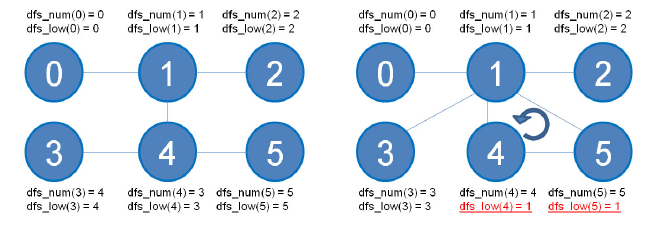
\includegraphics[width=0.9\textwidth]{../img/graph_articulation}
      \end{center}
    \begin{itemize}
    \item \structure{dfs\_num[]}: Recieves the number of the iteration
      when this node was reached for the first time;
    \item \structure{dfs\_low[]}: Recieves the lowest dfs\_num[] which
      can be reached if we start the DFS from here;
    \item For any neighbors $u,v$, if dfs\_low[$v$] >= dfs\_num[$u$],
      then $u$ is an articulation node.
    \end{itemize}
  }
\end{frame}

\begin{frame}[fragile]
  \frametitle{Tarjan's DFS variant for Articulation point (2)}
  \begin{center}
    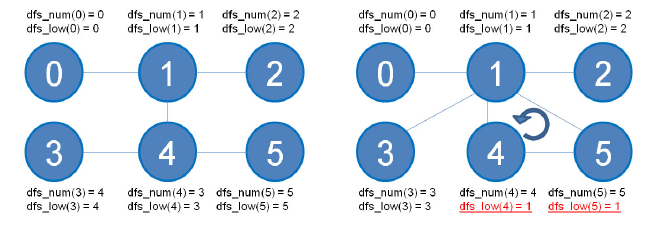
\includegraphics[width=0.6\textwidth]{../img/graph_articulation}
  \end{center}

{\tiny
  \begin{exampleblock}{}
\begin{verbatim}
void dfs_a(u){
   dfs_num[u] = dfs_low[u] = IterationCounter++;   // dfs_num[u] is a simple counter
   for (int i = 0; i < AdjList[u].size(); i++){
      v = AdjList[u][i];
      if (dfs_num[v] == UNVISITED) {
         dfs_parent[v] = u;                        // store parent
         if (u == 0) rootChildren++:               // special case for root node

         dfs_a(v);
         if (dfs_low[a] >= dfs_num[u])
            articulation_vertex[u] = true;
         dfs_low[u] = min(dfs_low[u],dfs_low[v])

      else if (v != dfs_parent[u])                 // found a cycle edge
         dfs_low[u] = min(dfs_low[u],dfs_num[v])
}}
\end{verbatim}
  \end{exampleblock}}
\end{frame}

\subsection{Strongly Connected Components}

\begin{frame}
  \frametitle{Strongly Connected Components (Directed Graph)}
  {\smaller
    \begin{block}{Problem Description}
      On a directed graph $G$, a Strongly Connected Component (SCC) is
      a subset $G'$ where for every pair of nodes $a,b \in G'$, there is both
      a path $a \rightarrow b$ and a path $b \rightarrow a$.
    \end{block}


\begin{columns}[t]
    \column{0.5\textwidth}
    \begin{exampleblock}{One CC}
      \vspace{0.1cm}
      \begin{center}
        \begin{tikzpicture}[scale=1.1,auto,swap]
          \node[vertex] (a) at (0,0) {};
          \node[vertex] (b) at (1,0) {};
          \node[vertex] (c) at (2,0) {};
          \node[vertex] (d) at (1,1) {};
          \node[vertex] (e) at (3,0) {};
          \node[vertex] (f) at (4,0) {};
          \node[vertex] (g) at (4,1) {};
          \node[vertex] (h) at (3,1) {};
          \draw[edge] (a) to (b);
          \draw[edge] (b) to (c);
          \draw[edge] (c) to (d);
          \draw[edge] (d) to (b);
          \draw[edge] (c) to (e);
          \draw[edge] (e) to (f);
          \draw[edge] (f) to (g);
          \draw[edge] (g) to (h);
          \draw[edge] (h) to (e);
        \end{tikzpicture}
      \end{center}
      \vspace{0.1cm}
    \end{exampleblock}
    \column{0.5\textwidth}
    \begin{exampleblock}{Three SCC}
      \vspace{0.1cm}
      \begin{center}
        \begin{tikzpicture}[scale=1.1,auto,swap]
          \tikzset{edge/.style = {->,>=latex'}}
          \node[vertex] (a) at (0,0) {};
          \node[blue vertex] (b) at (1,0) {};
          \node[blue vertex] (c) at (2,0) {};
          \node[blue vertex] (d) at (1,1) {};
          \node[red vertex] (e) at (3,0) {};
          \node[red vertex] (f) at (4,0) {};
          \node[red vertex] (g) at (4,1) {};
          \node[red vertex] (h) at (3,1) {};
          \draw[edge] (a) to (b);
          \draw[edge] (b) to (c);
          \draw[edge] (c) to (d);
          \draw[edge] (d) to (b);
          \draw[edge] (c) to (e);
          \draw[edge] (e) to (f);
          \draw[edge] (f) to (g);
          \draw[edge] (g) to (h);
          \draw[edge] (h) to (e);
        \end{tikzpicture}
      \end{center}
      \vspace{0.1cm}
    \end{exampleblock}
  \end{columns}
  }
\end{frame}

\begin{frame}
  \frametitle{Strongly Connected Components -- Algorithm}

  We can use a simple modification of the algorithm for bridges and
  articulation points:

  \begin{itemize}
    \item Every time we visit a new node, put that node in a stack $S$;
    \item When we finish visiting a node $i$, test if dfs\_num[$i$] == dfs\_min[$i$].
    \item If the above condition is true, $i$ is the root of the
      SCC. Pop all vertices in the stack as part of the SCC.
  \end{itemize}
\end{frame}

%%%%%%%%%%%%%%%%%%%%%%%%%%%%%%%%%%%%%%%%%%%%%%%

\section{Spanning Tree}
\subsection{Introduction}
\begin{frame}
  \frametitle{Minimum Spanning Trees (MST)}

  {\smaller
  \begin{block}{Definition}
    A \structure{Spanning Tree} is a subset $E'$ from graph $G$ so
    that all vertices are connected without cycles.

    \medskip

    A \structure{Minimum Spanning Tree} is a spanning tree where the
    sum of edge's weights is minimal.
  \end{block}
  }

  \begin{columns}[T]
    \column{0.3\textwidth}
    \begin{tikzpicture}[transform shape,label/.style={thin, draw=black, align=center,fill=white,font=\smaller},scale=1.1]
      \node[vertex] (a) at (0,0) {};
      \node[vertex] (b) at (1,1) {};
      \node[vertex] (c) at (2,0) {};
      \node[vertex] (d) at (1,-1) {};
      \node[vertex] (e) at (0,-2) {};
      \draw[edge] (a) -- node[label] {$4$} (b);
      \draw[edge] (b) -- node[label] {$2$} (c);
      \draw[edge] (a) -- node[label] {$4$} (c);
      \draw[edge] (a) -- node[label] {$6$} (d);
      \draw[edge] (c) -- node[label] {$8$} (d);
      \draw[edge] (a) -- node[label] {$6$} (e);
      \draw[edge] (d) -- node[label] {$9$} (e);
    \end{tikzpicture}
    \column{0.3\textwidth}
    \begin{tikzpicture}[transform shape,label/.style={thin, draw=black, align=center,fill=white,font=\smaller},scale=1.1]
      \node[vertex] (a) at (0,0) {};
      \node[vertex] (b) at (1,1) {};
      \node[vertex] (c) at (2,0) {};
      \node[vertex] (d) at (1,-1) {};
      \node[vertex] (e) at (0,-2) {};
      \draw[red edge] (a) -- node[label] {$4$} (b);
      \draw[red edge] (b) -- node[label] {$2$} (c);
      \draw[edge] (a) -- node[label] {$4$} (c);
      \draw[edge] (a) -- node[label] {$6$} (d);
      \draw[red edge] (c) -- node[label] {$8$} (d);
      \draw[edge] (a) -- node[label] {$6$} (e);
      \draw[red edge] (d) -- node[label] {$9$} (e);
    \end{tikzpicture}
    \column{0.3\textwidth}
    \begin{tikzpicture}[transform shape,label/.style={thin, draw=black, align=center,fill=white,font=\smaller},scale=1.1]
      \node[vertex] (a) at (0,0) {};
      \node[vertex] (b) at (1,1) {};
      \node[vertex] (c) at (2,0) {};
      \node[vertex] (d) at (1,-1) {};
      \node[vertex] (e) at (0,-2) {};
      \draw[red edge] (a) -- node[label] {$4$} (b);
      \draw[red edge] (b) -- node[label] {$2$} (c);
      \draw[edge] (a) -- node[label] {$4$} (c);
      \draw[red edge] (a) -- node[label] {$6$} (d);
      \draw[edge] (c) -- node[label] {$8$} (d);
      \draw[red edge] (a) -- node[label] {$6$} (e);
      \draw[edge] (d) -- node[label] {$9$} (e);
    \end{tikzpicture}
  \end{columns}
\end{frame}

\begin{frame}
  \frametitle{MST -- Use cases and Algorithms}
  {\small
  \begin{block}{Problems using MST}
    Problems using MST usually involve calculating the minimum costs
    of infrastructure such as roads or networks.

    \medskip

    Some variations may require you to find the \alert{maximum}
    spanning tree, or define some edges that \alert{must} be taken in advance.
  \end{block}

  \begin{exampleblock}{Algorithms for MST}
    The two main algorithms for calculating the MST are the
    \structure{Kruskal}'s algorithms and the \structure{Prim}'s
    algorithms.

    \medskip

    Both are greedy algorithms that add edges to the MST in weight order.
  \end{exampleblock}
    }
\end{frame}

\begin{frame}
  \frametitle{Kruskal's Algorithm}
  \begin{block}{Outline}
    Kruskal's algorithms sorts all edges by their weight, and try to
    add each edge to the MST, checking whether adding that edge would
    create a cycle.
  \end{block}

  \begin{columns}[T]
    \column{0.5\textwidth}
    \begin{enumerate}
    \item Sort all edges;
    \item If smallest edge does not create a cycle, add to MST;
    \item If smallest edge creates a cycle, remove it from list;
    \item Go to 2;
    \end{enumerate}
    \column{0.5\textwidth}
    \begin{tikzpicture}[transform shape,label/.style={thin, draw=black, align=center,fill=white,font=\smaller},scale=1.1]
      \node[vertex] (a) at (0,0) {};
      \node[vertex] (b) at (1,1) {};
      \node[vertex] (c) at (2,0) {};
      \node[vertex] (d) at (1,-1) {};
      \node[vertex] (e) at (0,-2) {};
      \draw[edge] (a) -- node[label] {$4$} (b);
      \draw[edge] (b) -- node[label] {$2$} (c);
      \draw[edge] (a) -- node[label] {$4$} (c);
      \draw[edge] (a) -- node[label] {$6$} (d);
      \draw[edge] (c) -- node[label] {$8$} (d);
      \draw[edge] (a) -- node[label] {$6$} (e);
      \draw[edge] (d) -- node[label] {$9$} (e);
      \draw<2->[red edge] (b) -- node[label] {$2$} (c);
      \draw<3->[red edge] (a) -- node[label] {$4$} (b);
      \draw<4->[black edge] (a) -- node[label] {$4$} (c);
      \draw<4->[red edge] (a) -- node[label] {$6$} (d);
      \draw<5->[red edge] (a) -- node[label] {$6$} (e);
    \end{tikzpicture}
  \end{columns}
\end{frame}

\begin{frame}[fragile]
  \frametitle{Kruskal's Algorithm -- Implementation}
{\smaller
\begin{exampleblock}{}
\begin{verbatim}
vector<pair<int, pair<int,int>> Edgelist;
sort(Edgelist.begin(),Edgelist.end());
int mst_cost = 0;
UnionFind UF(V);
  // note 1: Pair object has built-in comparison;
  // note 2: Need to implement UnionSet class;

for (int i = 0; i < Edgelist.size(); i++) {
   pair <int, pair <int,int>> front = Edgelist[i];
   if (!UF.isSameSet(front.second.first,
                     front.second.second)) {
      mst_cost += front.first;
      UF.unionSet(front.second.first,front.second.second)
   }}

cout << "MST Cost: " << mst_cost << "\n"
\end{verbatim}
\end{exampleblock}
}
\end{frame}

\begin{frame}
  \frametitle{Prim's Algorithm}
  {\small
  \begin{block}{Outline}
    Prim's algorith adds nodes to the MST one at a time, and keeps the
    edges connected to those nodes in a \structure{priority queue}. It
    then tests each edge in the priority queue to add more nodes to
    the MST, avoiding cycles.
  \end{block}

  \begin{columns}[T]
    \column{0.5\textwidth}
    \begin{enumerate}
    \item Add node 0 to MST;
    \item Add all edges from new node to Priority Queue;
    \item Visit smallest edge in Queue;
    \item If the edge leades to a new node, add it to MST;
    \item Add new edges to Queue;
    \item Go to 3;
    \end{enumerate}
    \column{0.5\textwidth}
    \begin{tikzpicture}[transform shape,label/.style={thin, draw=black, align=center,fill=white,font=\smaller},scale=1.1]
      \node[vertex] (a) at (0,0) {};
      \node[vertex] (b) at (1,1) {};
      \node[vertex] (c) at (2,0) {};
      \node[vertex] (d) at (1,-1) {};
      \node[vertex] (e) at (0,-2) {};
      \draw[edge] (a) -- node[label] {$4$} (b);
      \draw[edge] (b) -- node[label] {$2$} (c);
      \draw[edge] (a) -- node[label] {$4$} (c);
      \draw[edge] (a) -- node[label] {$6$} (d);
      \draw[edge] (c) -- node[label] {$8$} (d);
      \draw[edge] (a) -- node[label] {$6$} (e);
      \draw[edge] (d) -- node[label] {$9$} (e);
      \uncover<2->{
      \node[red vertex] (a1) at (0,0) {};
      \draw[black edge] (a) -- node[label] {$4$} (b);
      \draw[black edge] (a) -- node[label] {$4$} (c);
      \draw[black edge] (a) -- node[label] {$6$} (d);
      \draw[black edge] (a) -- node[label] {$6$} (e);
      }

      \uncover<3->{
        \node[red vertex] (c1) at (2,0) {};
        \draw[red edge] (a) -- node[label] {$4$} (c);
        \draw[black edge] (c) -- node[label] {$8$} (d);
        \draw[black edge] (b) -- node[label] {$2$} (c);
      }
      \uncover<4->{
        \node[red vertex] (b1) at (1,1) {};
        \draw[red edge] (b) -- node[label] {$2$} (c);
      }

      \uncover<5->{
        \node[red vertex] (d1) at (1,-1) {};
        \draw[red edge] (a) -- node[label] {$6$} (d);
        \draw[black edge] (d) -- node[label] {$9$} (e);
      }

      \uncover<6->{
        \node[red vertex] (e1) at (0,-2) {};
        \draw[red edge] (a) -- node[label] {$6$} (e);
      }
    \end{tikzpicture}
  \end{columns}
  }
\end{frame}

\begin{frame}[fragile]
  \frametitle{Prim's Algorithm -- Implementation}
{\smaller
\begin{exampleblock}{}
\begin{verbatim}
vector <int> taken;
priority_queue <pair <int,int>> pq;

void process (int v) {
   taken[v] = 1;
   for (int j = 0; j < (int)AdjList[v].size(); j++) {
      pair <int,int> ve = AdjList[v][j];
      if (!taken[ve.first])
         pq.push(pair <int,int> (-ve.second,-ve.second)
}}
taken.assign(V,0);
process(0);
mst_cost = 0;

while (!pq.empty()) {
  vector <int,int> pq.top(); pq.pop();
  u = -front.secont, w = -front.first;
  if (!taken[u]) mst_cost += w, process(u);
}
\end{verbatim}
\end{exampleblock}
}
\end{frame}

\subsection{Other MST Problems}

\begin{frame}
  \frametitle{MST variant 1 -- Maximum Spanning tree}

  {\smaller
    \begin{block}{}
      The \structure{Maximum Spanning Tree} variant requires the spanning
      tree to have maximum possible weight.

      \bigskip

      It is very easy to implement the Maximum MST by reversing the sort
      order of the edges (Kruskal), or the weighting of the priority Queue
      (Prim).
    \end{block}

  \medskip

  \begin{tikzpicture}[transform shape,label/.style={thin, draw=black, align=center,fill=white,font=\smaller},scale=1.1]
      \node[vertex] (a) at (0,0) {};
      \node[vertex] (b) at (1,1) {};
      \node[vertex] (c) at (0,2) {};
      \node[vertex] (d) at (-1,1) {};
      \node[vertex] (e) at (-2,0) {};
      \draw[red edge] (a) -- node[label] {$4$} (b);
      \draw[edge] (b) -- node[label] {$2$} (c);
      \draw[edge] (a) -- node[label] {$4$} (c);
      \draw[edge] (a) -- node[label] {$6$} (d);
      \draw[red edge] (c) -- node[label] {$8$} (d);
      \draw[red edge] (a) -- node[label] {$6$} (e);
      \draw[red edge] (d) -- node[label] {$9$} (e);
  \end{tikzpicture}}
\end{frame}

\begin{frame}
  \frametitle{MST variant 2 -- Minimum Spanning Subgraph, Forest}
  {\smaller
    \begin{block}{}
      In one importante variant of the MST, a subset of edges or
      vertices are pre-selected.

      \begin{itemize}
      \item In the case of pre-selected vertices, add them to the
        ``taken'' list in Kruskal's algorithm before starting;
      \item In the case of edges, add the end vertices to the
        ``taken'' list;
      \item What if you are given a \alert{number of Connected Components}?
      \end{itemize}
    \end{block}
    \begin{center}
      \begin{tikzpicture}[transform shape,label/.style={thin, draw=black, align=center,fill=white,font=\smaller},scale=1.1]
        \node[blue vertex] (a) at (0,0) {};
        \node[vertex] (b) at (1,1) {};
        \node[vertex] (c) at (2,2) {};
        \node[vertex] (d) at (3,1) {};
        \node[vertex] (e) at (4,0) {};
        \node[blue vertex] (f) at (4,2) {};
        \node[vertex] (g) at (5,0) {};
        \node[vertex] (h) at (6,2) {};
        \node[blue vertex] (i) at (6,1) {};
        \draw[red edge] (a) -- node[label] {$2$} (b);
        \draw[red edge] (a) -- node[label] {$1$} (d);
        \draw[edge] (d) -- node[label] {$4$} (c);
        \draw[edge] (d) -- node[label] {$8$} (e);
        \draw[edge] (d) -- node[label] {$3$} (f);
        \draw[red edge] (c) -- node[label] {$3$} (f);
        \draw[edge] (f) -- node[label] {$6$} (g);
        \draw[red edge] (e) -- node[label] {$4$} (g);
        \draw[red edge] (f) -- node[label] {$1$} (h);
        \draw[red edge] (g) -- node[label] {$3$} (i);
      \end{tikzpicture}
    \end{center}
  }
\end{frame}

\begin{frame}
  \frametitle{MST Variant 3 -- $n$th Best MST}
  {\smaller
  \begin{block}{Problem Definition}
    Consider that you can order MST by their costs: $G_1, G_2, \ldots,
    G_n$.  This variant asks you to calculate the $n^{th}$ best
    spanning tree.
  \end{block}

  \bigskip

  Basic Idea:
  \begin{itemize}
    \item Calculate the MST (using Kruskal or Prim);
    \item For every edge in the MST, remove that edge from the graph
      and calculate a new MST;
    \item The new MST with minimum weight is the $2^{nd}$ best MST;
  \end{itemize}
}
\end{frame}

\begin{frame}
  \frametitle{MST Variant 4 -- Min-max (or Max-min)}

  {\smaller

  \begin{center}
      \begin{tikzpicture}[transform shape,label/.style={thin, draw=black, align=center,fill=white,font=\tiny},scale=0.8]
        \node[red vertex] (a) at (0,0) {0};
        \node[vertex] (b) at (1,1) {1};
        \node[vertex] (c) at (1,-1) {2};
        \node[vertex] (d) at (2,0) {3};
        \node[vertex] (e) at (3,1) {4};
        \node[vertex] (f) at (3,-1) {5};
        \node[red vertex] (g) at (4,0) {6};
        \draw[red edge] (a) -- node[label] {$50$} (b);
        \draw[red edge] (a) -- node[label] {$60$} (c);
        \draw[edge] (b) -- node[label] {$120$} (d);
        \draw[edge] (b) -- node[label] {$90$} (e);
        \draw[red edge] (c) -- node[label] {$50$} (f);
        \draw[red edge] (d) -- node[label] {$80$} (f);
        \draw[red edge] (d) -- node[label] {$70$} (g);
        \draw[red edge] (e) -- node[label] {$40$} (g);
        \draw[edge] (f) -- node[label] {$140$} (g);
      \end{tikzpicture}
    \end{center}

  \begin{block}{Problem Definition}
    Given two vertices $i,j$, find a path $i \rightarrow j$ so that
    the cost of the most expensive edge is minimized;

    \medskip

    Another way to write this problem is: Find the cheapest path where
    the cost of the path is the cost of the most expensive edge.
  \end{block}

  \begin{exampleblock}{How to solve}
    The MST finds the path that connects all nodes while keeping the
    cost of individual edges minimal.

    \medskip

    To solve the minimax problem, we calculate the MST for $G$, and
    then find the path from $i$ to $j$ in the MST.
  \end{exampleblock}
  }
\end{frame}
